\begin{frame}\begin{center}
		\LARGE\textit{Theory of Human Capital}
\end{center}\end{frame}
%-------------------------------------------------------------------------------
%-------------------------------------------------------------------------------
\begin{frame}\textbf{Motivation}\vspace{0.3cm}
	\begin{figure}[htp]\centering
		\caption{Wage gains}\scalebox{0.35}
		{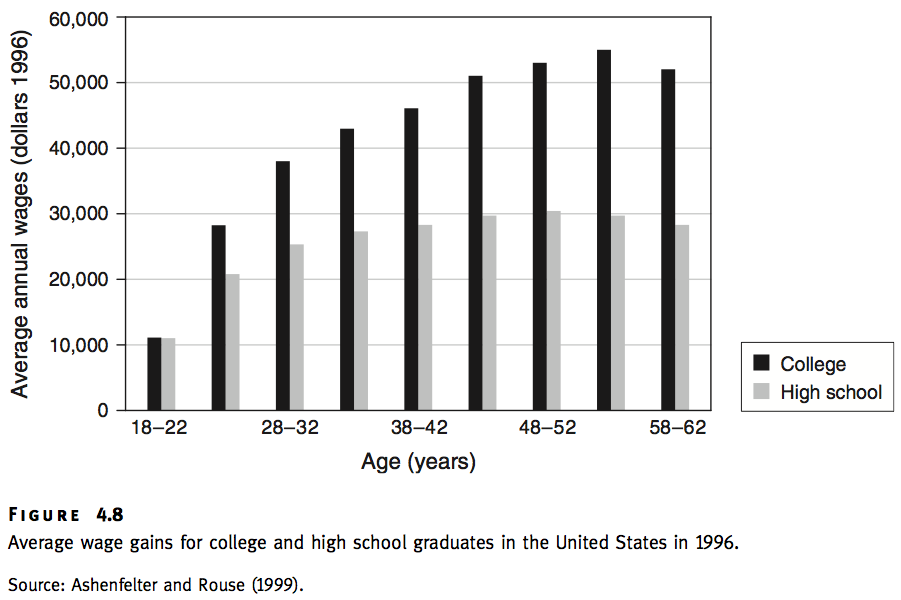
\includegraphics{fig-wage-gains}}
	\end{figure}
\end{frame}
%-------------------------------------------------------------------------------
%-------------------------------------------------------------------------------
\begin{frame}
We study the seminal Ben-Porath Model \cite{Ben-Porath.1967}.

\begin{align*}\begin{array}{l@{\qquad}l@{\qquad}l}
s(t) 	& \text{fraction devoted to training} \\
h(t)    & \text{stock of human capital} \\
w(t)	& \text{income} \\
\delta  & \text{depreciation of knowledge}
\end{array}\end{align*}
\end{frame}
%-------------------------------------------------------------------------------
%-------------------------------------------------------------------------------
\begin{frame}
The individual's objective is to maximize the discounted sum of wages over their life-cycle income.

\begin{align*}
\Omega = \int^T_0 w(t)\, e^{-r t} dt
\end{align*}
\end{frame}

\begin{frame}
Their economic environment is characterized by the production functions for income and human capital.

\begin{align*}
w(t)    & = A[1 - s(t)]h(t)dt \\
\dot{h} & = \theta g[s(t) h(t)] - \delta h(t) \qquad g^\prime > 0, g^{\prime\prime} < 0
\end{align*}

\end{frame}
%-------------------------------------------------------------------------------
%-------------------------------------------------------------------------------
\begin{frame}\textbf{Model Specification}\vspace{0.3cm}

We study the implementation in \citeA{Cahuc.2004}.

\begin{align*}\begin{array}{l@{\qquad}l@{\qquad}l}
	g(h(t), s(t)) = \left(h(t) s(t)\right)^{0.71} & & \\
	A = 0.75 & \delta = 0.06 & r = 0.05\\
	h_0 = 5 & T = 60 & \theta = 0.5
\end{array}\end{align*}

The implementation is available \href{http://bit.ly/2I2bMpb}{online}.
\end{frame}


\begin{frame}\begin{figure}[htp]\centering
\caption{Human capital production I}\label{Human capital production I}
\scalebox{0.35}{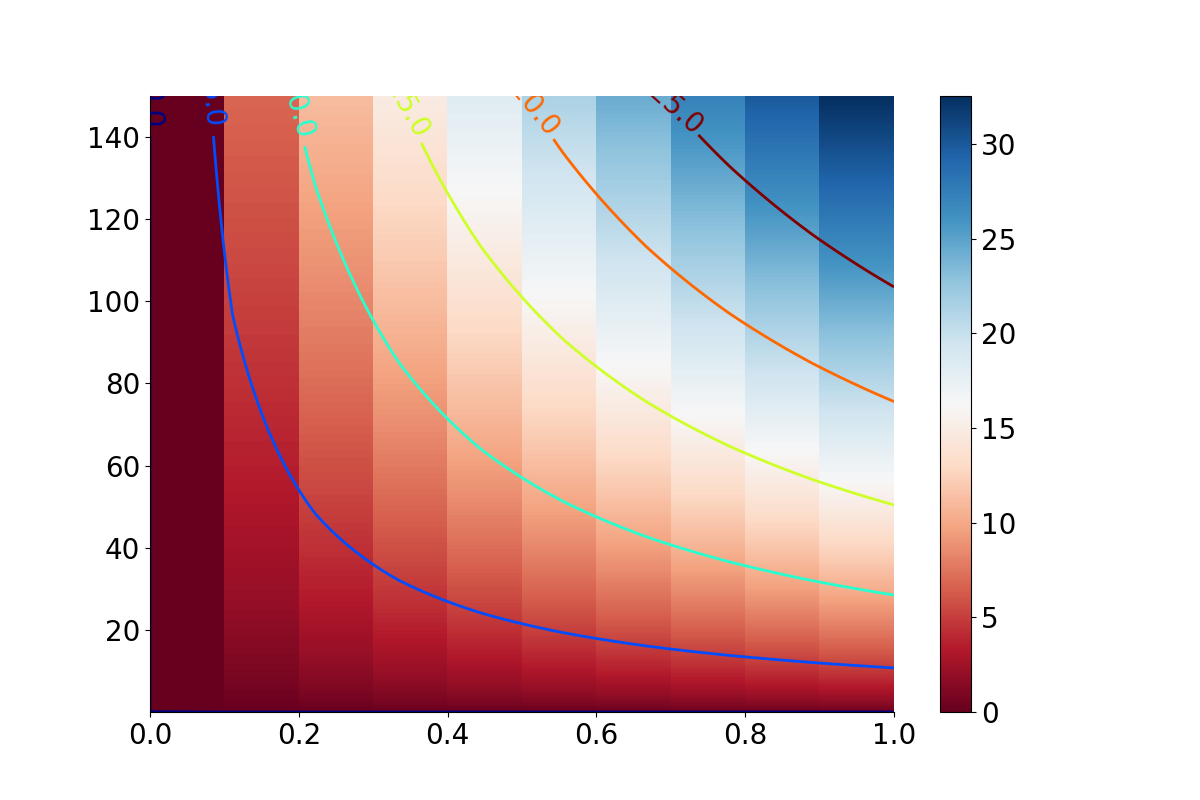
\includegraphics{fig-ben-porath-production-intensity}}
\end{figure}\end{frame}

\begin{frame}\begin{figure}[htp]\centering
\caption{Human capital production II}\label{Human capital production II}
\scalebox{0.35}{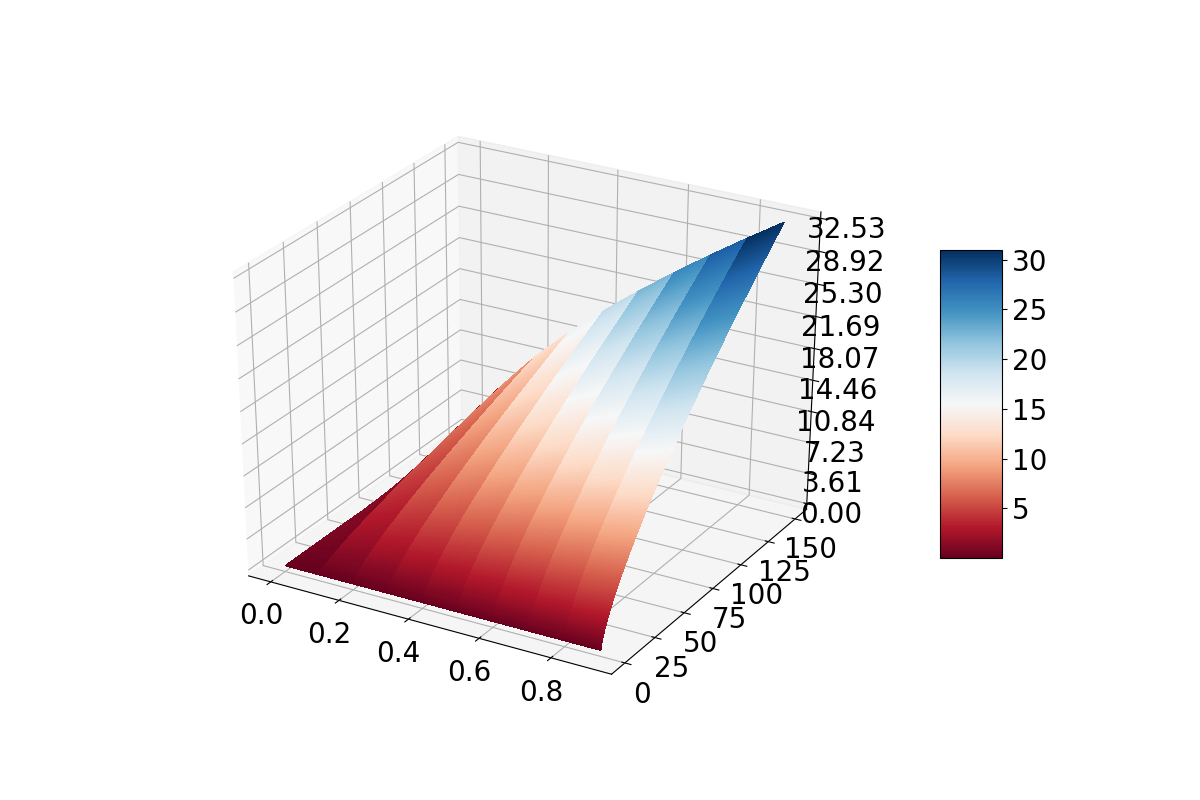
\includegraphics{fig-ben-porath-production-surface}}
\end{figure}\end{frame}

\begin{frame}\begin{figure}[htp]\centering
\caption{Income production}\label{Income production}
\scalebox{0.35}{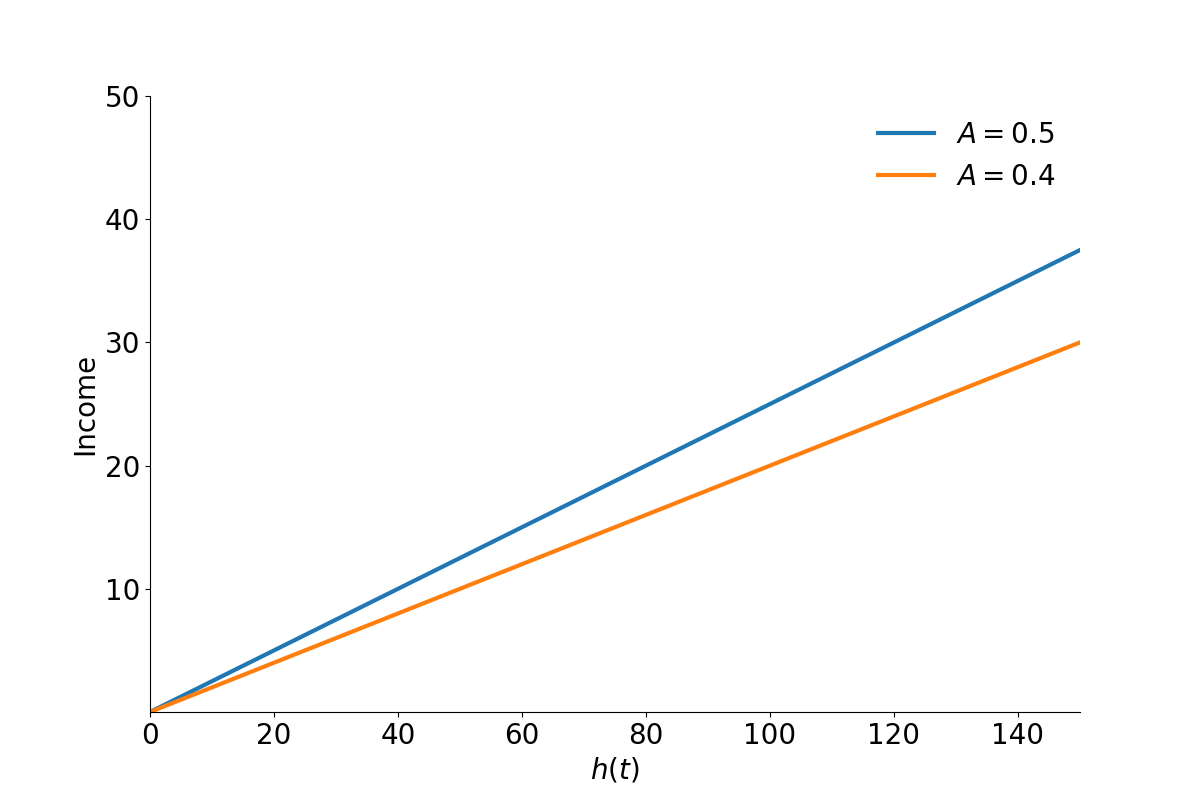
\includegraphics{fig-ben-porath-income}}
\end{figure}\end{frame}

\begin{frame}\begin{figure}[htp]\centering
\caption{Income over the life-cycle}\label{Income over the life-cycle}
\scalebox{0.35}{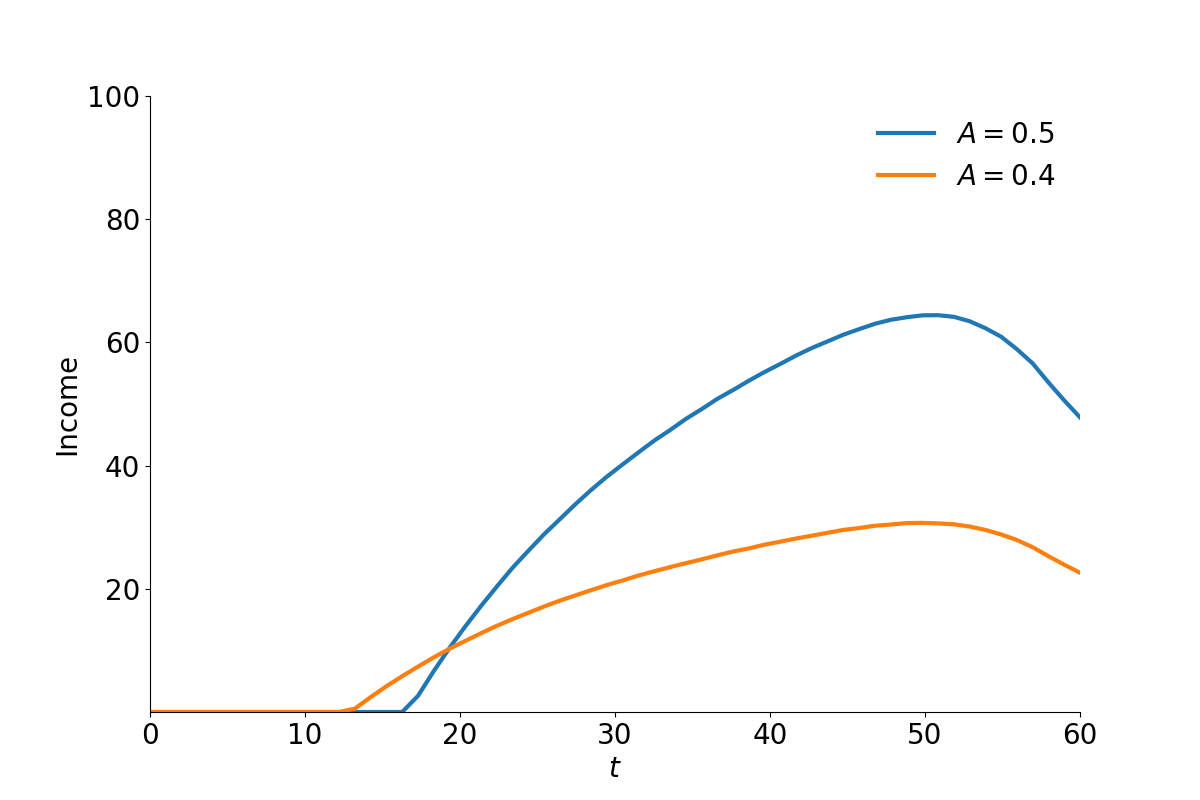
\includegraphics{fig-ben-porath-life-cycle-income}}
\end{figure}\end{frame}

\begin{frame}\begin{figure}[htp]\centering
\caption{Stock of human capital over the life-cycle}
\label{Stock of human capital over the life-cycle}
\scalebox{0.35}{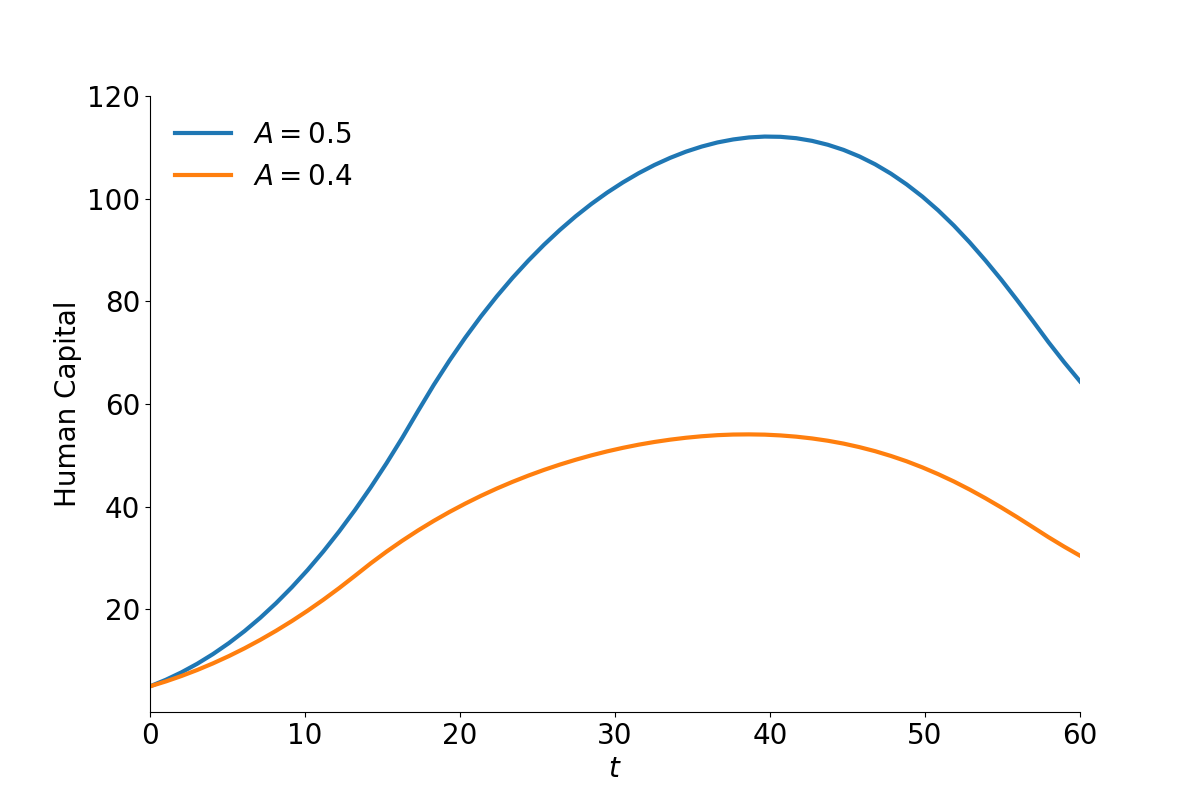
\includegraphics{fig-ben-porath-life-cycle-stock}}
\end{figure}\end{frame}

\begin{frame}\begin{figure}[htp]\centering
\caption{Human capital investment over the life-cycle}
\label{Human capital investment over the life-cycle}
\scalebox{0.35}{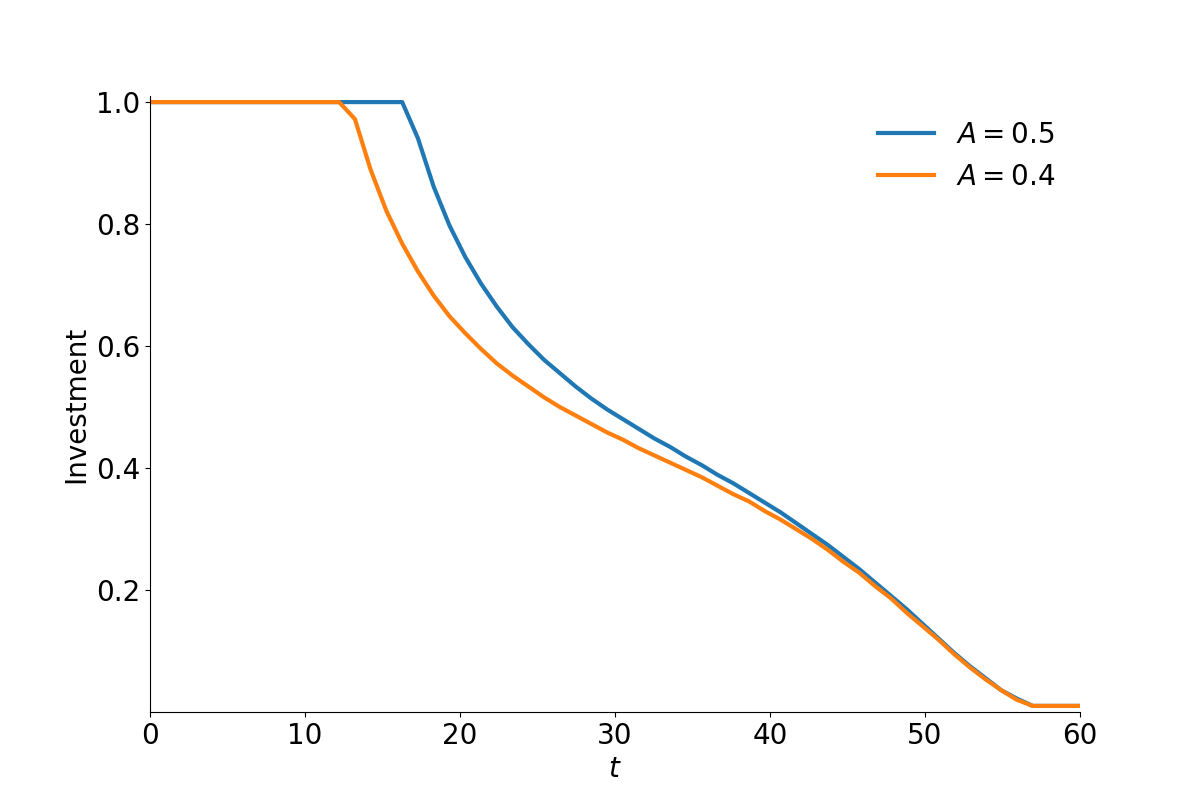
\includegraphics{fig-ben-porath-life-cycle-investment}}
\end{figure}\end{frame}
%-------------------------------------------------------------------------------
%-------------------------------------------------------------------------------
\begin{frame}\textbf{Extensions}\vspace{0.3cm}

\citeA{Weiss.1986} reviews a host of alternative extensions to the basic model.\\

\begin{itemize}\setlength\itemsep{1em}
\item general versus specific training
\item hours worked
\item uncertainty
\item $\hdots$
\end{itemize}

\end{frame}
